% ============================================================
% Fundamentos, práticas e experiências da IA na comunicação
% Template de apresentação (Beamer) para o seminário do Cogecom Sudeste / XVIII Secom
%
% Compilar com: lualatex seminario_ia_comunicacao.tex   (recomendado)
%           ou: xelatex seminario_ia_comunicacao.tex
%           ou: pdflatex seminario_ia_comunicacao.tex   (usa fonte alternativa, sem Poppins)
%
% Estrutura pensada para o framework 4D do curso AI Fluency (Anthropic Academy,
% Feller & Dakan): Delegação, Descrição, Discernimento, Diligência.
% Seção "Ferramentas" é o centro da apresentação (mais slides), "Possibilidades"
% tem mais peso do que "Limites", como combinado.
%
% Os blocos marcados com [PREENCHER] são placeholders de propósito: exemplos de
% ferramentas e casos reais da comunicação você conhece melhor do que eu.
% ============================================================

\documentclass[aspectratio=169,11pt]{beamer}
\newcommand{\hl}[1]{\textcolor{terracota}{#1}}
\usepackage{iftex}
\ifPDFTeX
  \usepackage[utf8]{inputenc}
  \usepackage[T1]{fontenc}
  \usepackage{lmodern}
\else
  \usepackage{fontspec}
  \IfFontExistsTF{Poppins}{%
    \setmainfont{Poppins}[
      UprightFont = *-Regular,
      BoldFont = *-Medium,
      ItalicFont = *-Italic,
      BoldItalicFont = *-MediumItalic
    ]
  }{%
    \setmainfont{Latin Modern Sans}
  }
\fi

\usepackage[brazil]{babel}
\usepackage{tikz}
\usepackage{xcolor}
\usepackage{booktabs}
\usepackage{tcolorbox}
\usepackage{pifont}
\usepackage{hyperref}

\tcbuselibrary{skins,breakable}

% ---------------------------------------------------------------
% Paleta (azul marinho + terracota, seguindo o estilo já usado por
% Rodrigo em outros materiais). Só duas cores de destaque + cinzas.
% ---------------------------------------------------------------
\definecolor{navy}{RGB}{16,32,58}
\definecolor{terracota}{RGB}{212,116,66}
\definecolor{graytxt}{RGB}{102,102,102}
\definecolor{lightgray}{RGB}{225,225,225}

% ---------------------------------------------------------------
% Tema base: totalmente plano, sem barra lateral, sem símbolos de
% navegação, sem caixas de título coloridas cheias.
% ---------------------------------------------------------------
\usetheme{default}
\usecolortheme{default}
\setbeamertemplate{navigation symbols}{}
\setbeamercolor{background canvas}{bg=white}
\setbeamercolor{normal text}{fg=navy}
\setbeamercolor{frametitle}{fg=navy}
\setbeamercolor{structure}{fg=navy}
\setbeamercolor{alerted text}{fg=terracota}
\setbeamerfont{frametitle}{series=\bfseries,size=\Large}
\setbeamerfont{title}{series=\bfseries}

% título de frame: texto em navy + traço fino terracota embaixo,
% sem caixa colorida de fundo
\setbeamertemplate{frametitle}{
  \vspace{0.35cm}
  \hspace{0.1cm}\usebeamerfont{frametitle}\usebeamercolor[fg]{frametitle}\insertframetitle\\[0.12cm]
  \hspace{0.1cm}\textcolor{terracota}{\rule{2.1cm}{1.4pt}}
  \vspace{0.15cm}
}

% rodapé discreto: seção corrente à esquerda, contador à direita
\setbeamertemplate{footline}{
  \begin{beamercolorbox}[wd=\paperwidth,ht=0.5cm,dp=0.15cm,leftskip=0.4cm,rightskip=0.4cm]{normal text}
    \color{graytxt}\tiny\insertsectionhead
    \hfill
    \color{graytxt}\tiny IA na comunicação
    \hfill
    \color{graytxt}\tiny\insertframenumber\,/\,\inserttotalframenumber
  \end{beamercolorbox}
}

% marcadores de lista: quadrado terracota no nível 1, traço navy no nível 2
\setbeamertemplate{itemize item}{{\rule{4.2pt}{4.2pt}}}
\setbeamertemplate{itemize subitem}{\textcolor{navy}{\textendash}}
\addtobeamertemplate{itemize/enumerate body begin}{\setlength{\itemsep}{4pt}}{}

\setbeamertemplate{caption}[numbered]

% ---------------------------------------------------------------
% Caixas minimalistas (barra fina lateral, sem preenchimento pesado)
% ---------------------------------------------------------------
\newtcolorbox{notebox}[1]{
  enhanced, breakable, colback=white, colframe=white,
  boxrule=0pt, leftrule=2.6pt, colframe=navy,
  arc=0pt, left=8pt, right=6pt, top=6pt, bottom=6pt,
  before upper={\bfseries\color{navy}#1\par\vspace{3pt}\normalfont\color{navy}}
}

\newtcolorbox{alertbox}[1]{
  enhanced, breakable, colback=white, colframe=white,
  boxrule=0pt, leftrule=2.6pt, colframe=terracota,
  arc=0pt, left=8pt, right=6pt, top=6pt, bottom=6pt,
  before upper={\bfseries\color{terracota}#1\par\vspace{3pt}\normalfont\color{navy}}
}

% ---------------------------------------------------------------
% Macro reutilizável para os slides de ferramentas: categoria de
% ferramenta, uma linha de contexto, lista de bom uso e de mau uso.
% Use este comando para acrescentar quantas categorias quiser.
% ---------------------------------------------------------------
\newcommand{\ferramentaframe}[4]{%
\begin{frame}{#1}
  {\small\color{graytxt} #2}
  \vspace{0.25cm}
  \begin{columns}[T,onlytextwidth]
    \begin{column}{0.485\textwidth}
      \begin{notebox}{\ding{51}\ \ Bom uso}
        \small
        \begin{itemize}
          #3
        \end{itemize}
      \end{notebox}
    \end{column}
    \begin{column}{0.485\textwidth}
      \begin{alertbox}{\ding{55}\ \ Mau uso}
        \small
        \begin{itemize}
          #4
        \end{itemize}
      \end{alertbox}
    \end{column}
  \end{columns}
\end{frame}
}

% ---------------------------------------------------------------
% Macro para os slides separadores de seção (fundo navy, título
% grande em branco, traço terracota).
% ---------------------------------------------------------------
\newcommand{\dividerframe}[2]{%
\begin{frame}[plain]
\begin{tikzpicture}[remember picture, overlay]
  \fill[navy] (current page.south west) rectangle (current page.north east);
  \node[anchor=west, align=left, text width=0.85\paperwidth] at ([xshift=1cm]current page.west) {
    \hyphenpenalty=10000\exhyphenpenalty=10000
    \textcolor{terracota}{\rule{1.4cm}{2pt}}\\[0.45cm]
    {\color{white}\fontsize{24}{28}\selectfont\bfseries #1}\\[0.3cm]
    {\color{white!65!navy}\normalsize #2}
  };
\end{tikzpicture}
\end{frame}
}

\hypersetup{colorlinks=true, linkcolor=navy, urlcolor=terracota}

\title{Fundamentos, práticas e experiências da Inteligência Artificial na comunicação}
\author{Rodrigo Cesar Pedrosa Silva}
\institute{Coordenador do Bacharelado em Inteligência Artificial, UFOP}
\date{10 de setembro de 2026}

\begin{document}

% =========================================================
% CAPA
% =========================================================
\begin{frame}[plain]
  \vspace{0.3cm}
  {\color{graytxt}\small Cogecom Sudeste \ \textbullet\ \ XVIII Secom \ \textbullet\ \ UFOP}\\[0.45cm]
  \begin{minipage}[t]{0.86\paperwidth}
    \raggedright\hyphenpenalty=10000\exhyphenpenalty=10000
    {\color{navy}\fontsize{22}{26}\selectfont\bfseries Fundamentos, práticas e experiências da Inteligência Artificial (na comunicação)}
  \end{minipage}\\[0.35cm]
  \textcolor{terracota}{\rule{3cm}{2pt}}\\[0.35cm]
  % Subtítulo-tese: sugestão que alude à seção de ferramentas via o framework 4D.
  % Ajuste para a formulação que preferir antes de apresentar.

  {\color{graytxt}\small \textbf{Prof. Rodrigo Cesar Pedrosa Silva} \\ 
  Coordenador do Bacharelado em Inteligência Artificial, UFOP\\ 
  Departamento de Computação - Instituto de Ciências Exatas e Biológicas (ICEB)\\
   CSILab - Laboratório de Computação de Sistemas Inteligentes \\
  10 de setembro de 2026}

\end{frame}

\begin{frame}{Disclaimer}
  \begin{itemize}
    \item Esta apresentação \hl{não é uma vitrine de ferramentas}
    \item O foco aqui são \hl{conceitos e fundamentos}
    \item Princípios que valem para a ferramenta que você usa hoje e para a que vai substituí-la amanhã
    \item Esses fundamentos não ficam somente na teoria
  \end{itemize}
\end{frame}

% =========================================================
\section{Fluência em IA}
% =========================================================
\dividerframe{Fluência em IA}{AI Fluency - Claude Academy \\ Rick Dakan - Ringling College of Art and Design}

\begin{frame}{Por que fluência?}
  \begin{itemize}
    \item Modelos, ferramentas e prompts \hl{mudam o tempo inteiro} 
    \item Como escrever um bom prompt para uma tarefa específica envelhece rápido 
    \begin{itemize}
      \item Exemplo: Quebrar a tarefa em subtarefas
    \end{itemize}
    \item \hl{Quais princípios devem guiar a nossa interação com a IA?}
    \item \hl{Saber usar bem} a IA \hl{de forma responsável}
  \end{itemize}

  \vspace{0.3cm}
  \begin{notebox}{Definição}
    \small Fluência em IA é interagir com sistemas de IA de forma eficaz, eficiente, ética e segura, e adaptar essa forma de interagir conforme a tecnologia muda.
  \end{notebox}
\end{frame}

\begin{frame}{Três formas de trabalhar com IA}
  \begin{itemize}
    \item \textbf{Automação}: a IA executa uma tarefa bem definida no seu lugar (transcrever, resumir, formatar)
    \item \textbf{Aumento}: você e a IA trabalham juntos, em ida e volta, para pensar melhor (rascunhar, revisar, analisar, explorar alternativas)
    \item \textbf{Agência}: a IA conduz várias etapas de um processo com autonomia, sob supervisão sua (pesquisar, redigir e revisar um material em sequência)
  \end{itemize}
\end{frame}


% \begin{frame}{Capacidades e limites, lado a lado}
%   \begin{columns}[T,onlytextwidth]
%     \begin{column}{0.485\textwidth}
%       \begin{notebox}{O que a IA generativa faz bem}
%         \small
%         \begin{itemize}
%           \item Gerar variações de texto e formato rapidamente
%           \item Sintetizar grandes volumes de informação
%           \item Manter consistência de estilo e tom
%           \item Adaptar um mesmo conteúdo para públicos diferentes
%         \end{itemize}
%       \end{notebox}
%     \end{column}
%     \begin{column}{0.485\textwidth}
%       \begin{alertbox}{Onde ela ainda falha}
%         \small
%         \begin{itemize}
%           \item Não verifica fatos, apenas prevê texto plausível
%           \item Não tem acesso automático ao contexto institucional
%           \item Não responde por decisões éticas ou editoriais
%           \item Erra com mais frequência do que aparenta
%         \end{itemize}
%       \end{alertbox}
%     \end{column}
%   \end{columns}
% \end{frame}

% =========================================================
\section{O framework das quatro competências}
% =========================================================
\dividerframe{O framework das quatro competências}{Delegação, Descrição, Discernimento, Diligência}

\begin{frame}{Competências para a fluência em IA}
  \begin{itemize}
    \item \textbf{Delegação}: \hl{o que passar para a IA}, e o que continua sendo trabalho humano
    \item \textbf{Descrição}: \hl{como comunicar o que se quer}, com contexto e critérios
    \item \textbf{Discernimento}: \hl{como avaliar} criticamente o que a IA devolveu
    \item \textbf{Diligência}: \hl{quem responde pelo resultado final}
  \end{itemize}
\end{frame}


\begin{frame}{Delegação}
  \begin{notebox}{Definição}
    \small Ter visão de conjunto antes de dividir o trabalho: o que você quer alcançar, o que só uma pessoa deve fazer, e onde a IA realmente ajuda.
  \end{notebox}

  \textbf{Pergunta-guia:} esta tarefa exige julgamento humano, ou é mecânica o suficiente para delegar?

  \begin{alertbox}{Cuidado}
    \small Delegar não é apenas transferir a tarefa: sem um objetivo claro, delegação vira terceirização sem controle.
  \end{alertbox}

  \begin{itemize}
    \item Delegar o levantamento e o rascunho, não a decisão final do que vai ao ar
  \end{itemize}
\end{frame}

\begin{frame}{Descrição}
  \begin{notebox}{Definição}
    \small Ter uma conversa com contexto suficiente sobre o que se quer, como a IA deve abordar a tarefa, e o tom esperado.
  \end{notebox}
  \textbf{Pergunta-guia:} Se eu desse essas mesmas instruções a um estagiário novo e esperaria um bom resultado? \hl{A IA não lê nossos pensamentos}
  
  \begin{alertbox}{A diferença}
    \small ``Escreva uma nota'' e ``escreva uma nota de até 200 palavras, tom institucional, para veículos locais, evitando jargão técnico'' geram resultados muito diferentes.
  \end{alertbox}

  \begin{itemize}
    \item Público, tom, tamanho, o que evitar, exemplos 
  \end{itemize}
\end{frame} 

\begin{frame}{Discernimento}
  \begin{notebox}{Definição}
    \small Avaliar criticamente o que a IA devolveu, com a expertise que só você tem no assunto: o que aproveitar, o que ajustar, o que descartar por completo.
  \end{notebox}
  \vspace{0.1cm}
  \textbf{Pergunta-guia:} eu assinaria embaixo disso?
  \vspace{0.1cm}
  \begin{alertbox}{Ponto central}
    \small É a sua expertise no assunto que permite perceber quando a IA está errada com segurança.
  \end{alertbox}
  \vspace{0.1cm}
  \begin{itemize}
    \item Na comunicação: fatos, números e citações sempre checados, e a pergunta final: isso está alinhado com a linha editorial e realmente ajuda a avançar? 
  \end{itemize}
\end{frame}

\begin{frame}{Diligência}
  \begin{notebox}{Definição}
    \small Assumir a responsabilidade pelo resultado final: pelo que foi publicado, pelo que foi automatizado, pelas consequências.
  \end{notebox}

  \textbf{Pergunta-guia:} se isso der errado depois de publicado, quem responde por essa decisão? A IA não assina a nota oficial, a assessoria assina, e é ela quem responde pelo que foi publicado

  \begin{alertbox}{Um cuidado concreto}
    \small Dados sensíveis compartilhados com uma ferramenta de IA: onde ficam armazenados, e quem mais tem acesso a eles?
  \end{alertbox}

\end{frame}

\begin{frame}{O Framework 4D}
\begin{center}
\resizebox{0.82\linewidth}{!}{%
\begin{tikzpicture}[
  compnode/.style={rectangle, rounded corners=3pt, fill=navy,
    minimum width=3.1cm, minimum height=1.05cm, align=center, inner sep=4pt},
  arr/.style={<->, navy, line width=1.1pt}
]

% quatro nós: topo, baixo, esquerda, direita
\node[compnode] (delegacao) at (0,1.7) {\color{white}\bfseries\footnotesize Delegação};
\node[compnode] (diligencia) at (0,-1.7) {\color{white}\bfseries\footnotesize Diligência};
\node[compnode] (descricao) at (-4.3,0) {\color{white}\bfseries\footnotesize Descrição};
\node[compnode] (discernimento) at (4.3,0) {\color{white}\bfseries\footnotesize Discernimento};

% duas retas cruzando o centro
\draw[arr] (delegacao) -- (diligencia);
\draw[arr] (descricao) -- (discernimento);

% quatro curvas ligando cantos adjacentes
\draw[arr] (delegacao) to[bend right=25] (descricao);
\draw[arr] (delegacao) to[bend left=25] (discernimento);
\draw[arr] (diligencia) to[bend left=25] (descricao);
\draw[arr] (diligencia) to[bend right=25] (discernimento);

\end{tikzpicture}
}
\end{center}
\vspace{0.2cm}
{\small\color{graytxt}\centering As quatro competências são interconectadas: cada uma influencia e é influenciada pelas outras.\par}
\end{frame}

% ---------------------------------------------------------------
% Exercício prático: aplicando o 4D a um projeto de comunicação.
% Uma pergunta por competência, com opções para votação ao vivo
% (mão levantada, ou ferramenta de enquete). Os votos não têm
% resposta certa: servem para comparar critérios da equipe.
% ---------------------------------------------------------------
\dividerframe{Exemplo: aplicando o 4D}{Um projeto de comunicação, quatro decisões}

\begin{frame}{O projeto: Mostra de Profissões}
  \begin{notebox}{O cenário}
    \small Você está trabalhando com um assistente de IA para redigir uma série de posts de Instagram para a campanha de marketing da mostra de profissões da universidade.
  \end{notebox}
  \vspace{0.3cm}
\end{frame}

\begin{frame}{Delegação}
  \begin{notebox}{Pergunta}
    \small Quais aspectos deste projeto você faria sozinho, e quais delegaria à IA?
  \end{notebox}
  \vspace{0.3cm}
  \begin{itemize}
    \item[\textbf{\color{terracota}A}] A IA redige os posts inteiros, eu só reviso antes de publicar
    \item[\textbf{\color{terracota}B}] Escrevo a mensagem central eu mesmo, delego só as variações de formato para cada rede
    \item[\textbf{\color{terracota}C}] Peço um brainstorm de ideias e ângulos à IA, mas escrevo o texto final eu mesmo
    \item[\textbf{\color{terracota}D}] Faço tudo sozinho, uso a IA só para revisão ortográfica
  \end{itemize}
\end{frame}

\begin{frame}{Descrição}
  \begin{notebox}{Pergunta}
    \small Como você comunicaria à IA sua visão para o tom, o propósito e os critérios de sucesso da campanha?
  \end{notebox}
  \vspace{0.3cm}
  \begin{itemize}
    \item[\textbf{\color{terracota}A}] Um pedido direto: ``escreva posts animados divulgando a mostra de profissões''
    \item[\textbf{\color{terracota}B}] Um briefing com público-alvo, tom de voz, datas, chamada para ação e exemplos de posts que já funcionaram
    \item[\textbf{\color{terracota}C}] Uma conversa em várias rodadas: começo simples e vou refinando o tom conforme a IA responde
    \item[\textbf{\color{terracota}D}] Um documento de identidade de marca da universidade, anexado à conversa
  \end{itemize}
\end{frame}

\begin{frame}{Discernimento}
  \begin{notebox}{Pergunta}
    \small Se você só pudesse checar um critério antes de publicar os posts da IA, qual seria?
  \end{notebox}
  \vspace{0.3cm}
  \begin{itemize}
    \item[\textbf{\color{terracota}A}] Os fatos e informações práticas estão corretos (datas, locais, cursos)
    \item[\textbf{\color{terracota}B}] O tom soa como a voz da universidade, não como um texto genérico de IA
    \item[\textbf{\color{terracota}C}] O post tem potencial real de engajamento (curtidas, compartilhamentos, cliques)
    \item[\textbf{\color{terracota}D}] A mensagem está alinhada com os valores e a política de comunicação da instituição
  \end{itemize}
\end{frame}

\begin{frame}{Diligência}
  \begin{notebox}{Pergunta}
    \small Qual desses cuidados de transparência e responsabilidade é mais urgente para a sua equipe adotar agora?
  \end{notebox}
  \vspace{0.3cm}
  \begin{itemize}
    \item[\textbf{\color{terracota}A}] Avisar publicamente que os posts foram feitos com apoio de IA
    \item[\textbf{\color{terracota}B}] Garantir que uma pessoa da equipe revise e assine a aprovação final antes de publicar
    \item[\textbf{\color{terracota}C}] Verificar se imagens geradas por IA não simulam pessoas ou situações reais sem identificação
    \item[\textbf{\color{terracota}D}] Registrar internamente quais partes foram feitas com IA, para eventuais questionamentos futuros
  \end{itemize}
\end{frame}

% =========================================================
\section{Fundamentos de IA generativa}
% =========================================================
\dividerframe{Fundamentos de IA generativa}{Capacidades e Limitações}
% ---------------------------------------------------------------
% Fundamentos de IA generativa: o que é, como surgiu, como
% funciona por baixo do capô, e o que torna isso poderoso.
% ---------------------------------------------------------------
\begin{frame}{O que é IA generativa}
  \begin{notebox}{A diferença}
    \small IA tradicional analisa e classifica dados existentes (dizer se um e-mail é spam). IA generativa cria conteúdo novo, que não existia antes (escrever um e-mail inteiro).
  \end{notebox}
  \vspace{0.3cm}
  \begin{itemize}
    \item Modelos de linguagem (LLMs), como o Claude e GPT, são o tipo mais conhecido de IA generativa
    \item ``Modelo de linguagem'': treinado para prever e gerar linguagem humana
    \item ``Grande'': contém bilhões de parâmetros, os valores que moldam como o modelo processa informação
  \end{itemize}
\end{frame}


\begin{frame}{Como o modelo aprende}
  \begin{columns}[c]
    \begin{column}{0.5\textwidth}
      \begin{notebox}{Pré-treinamento}
        \small O modelo lê bilhões de exemplos de texto e aprende a prever a próxima palavra. Repetindo isso muitas vezes, constrói uma espécie de mapa estatístico da linguagem e do conhecimento.
      \end{notebox}
    \end{column}
    \begin{column}{0.5\textwidth}
      \centering
      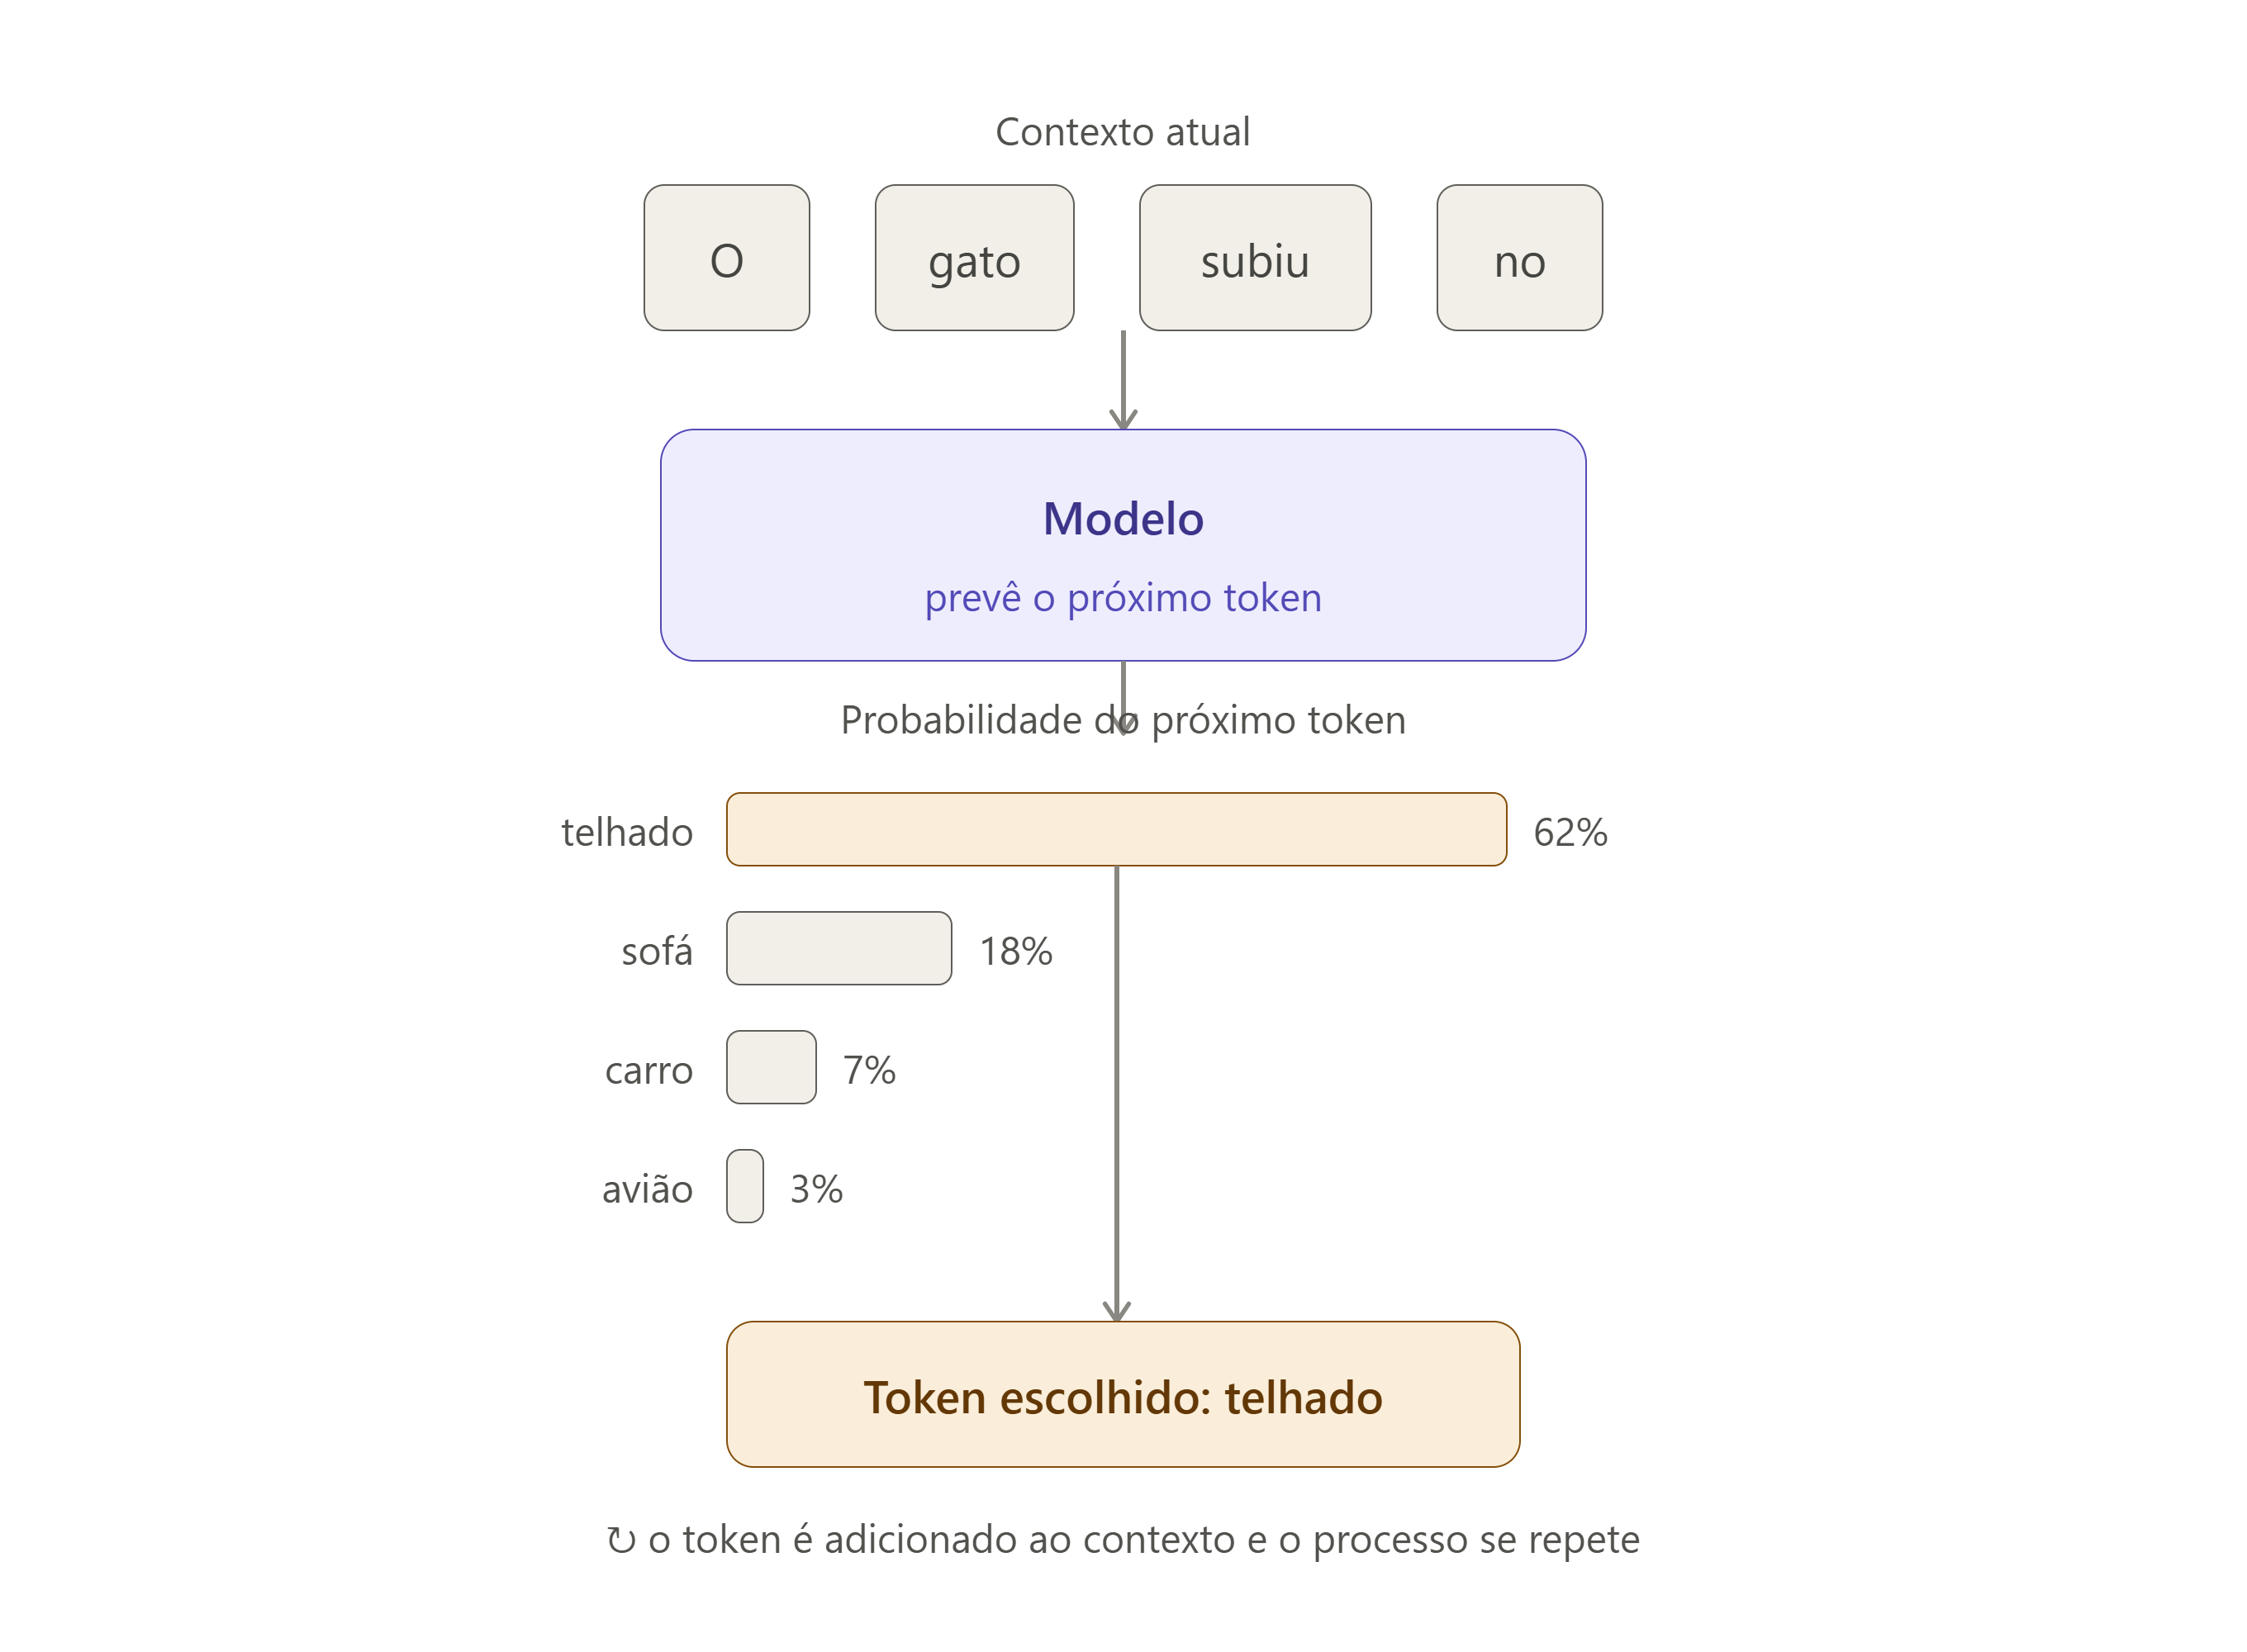
\includegraphics[scale=0.1]{next_token_prediction.png}
    \end{column}
  \end{columns}
\end{frame}


\begin{frame}{Como o modelo aprende}
  \begin{columns}[c]
    \begin{column}{0.5\textwidth}
      \begin{notebox}{Ajuste fino}
    \small Depois, o modelo aprende a seguir instruções, dar respostas úteis e evitar conteúdo nocivo, com apoio de feedback humano.
  \end{notebox}
    \end{column}
    \begin{column}{0.5\textwidth}
      \centering
      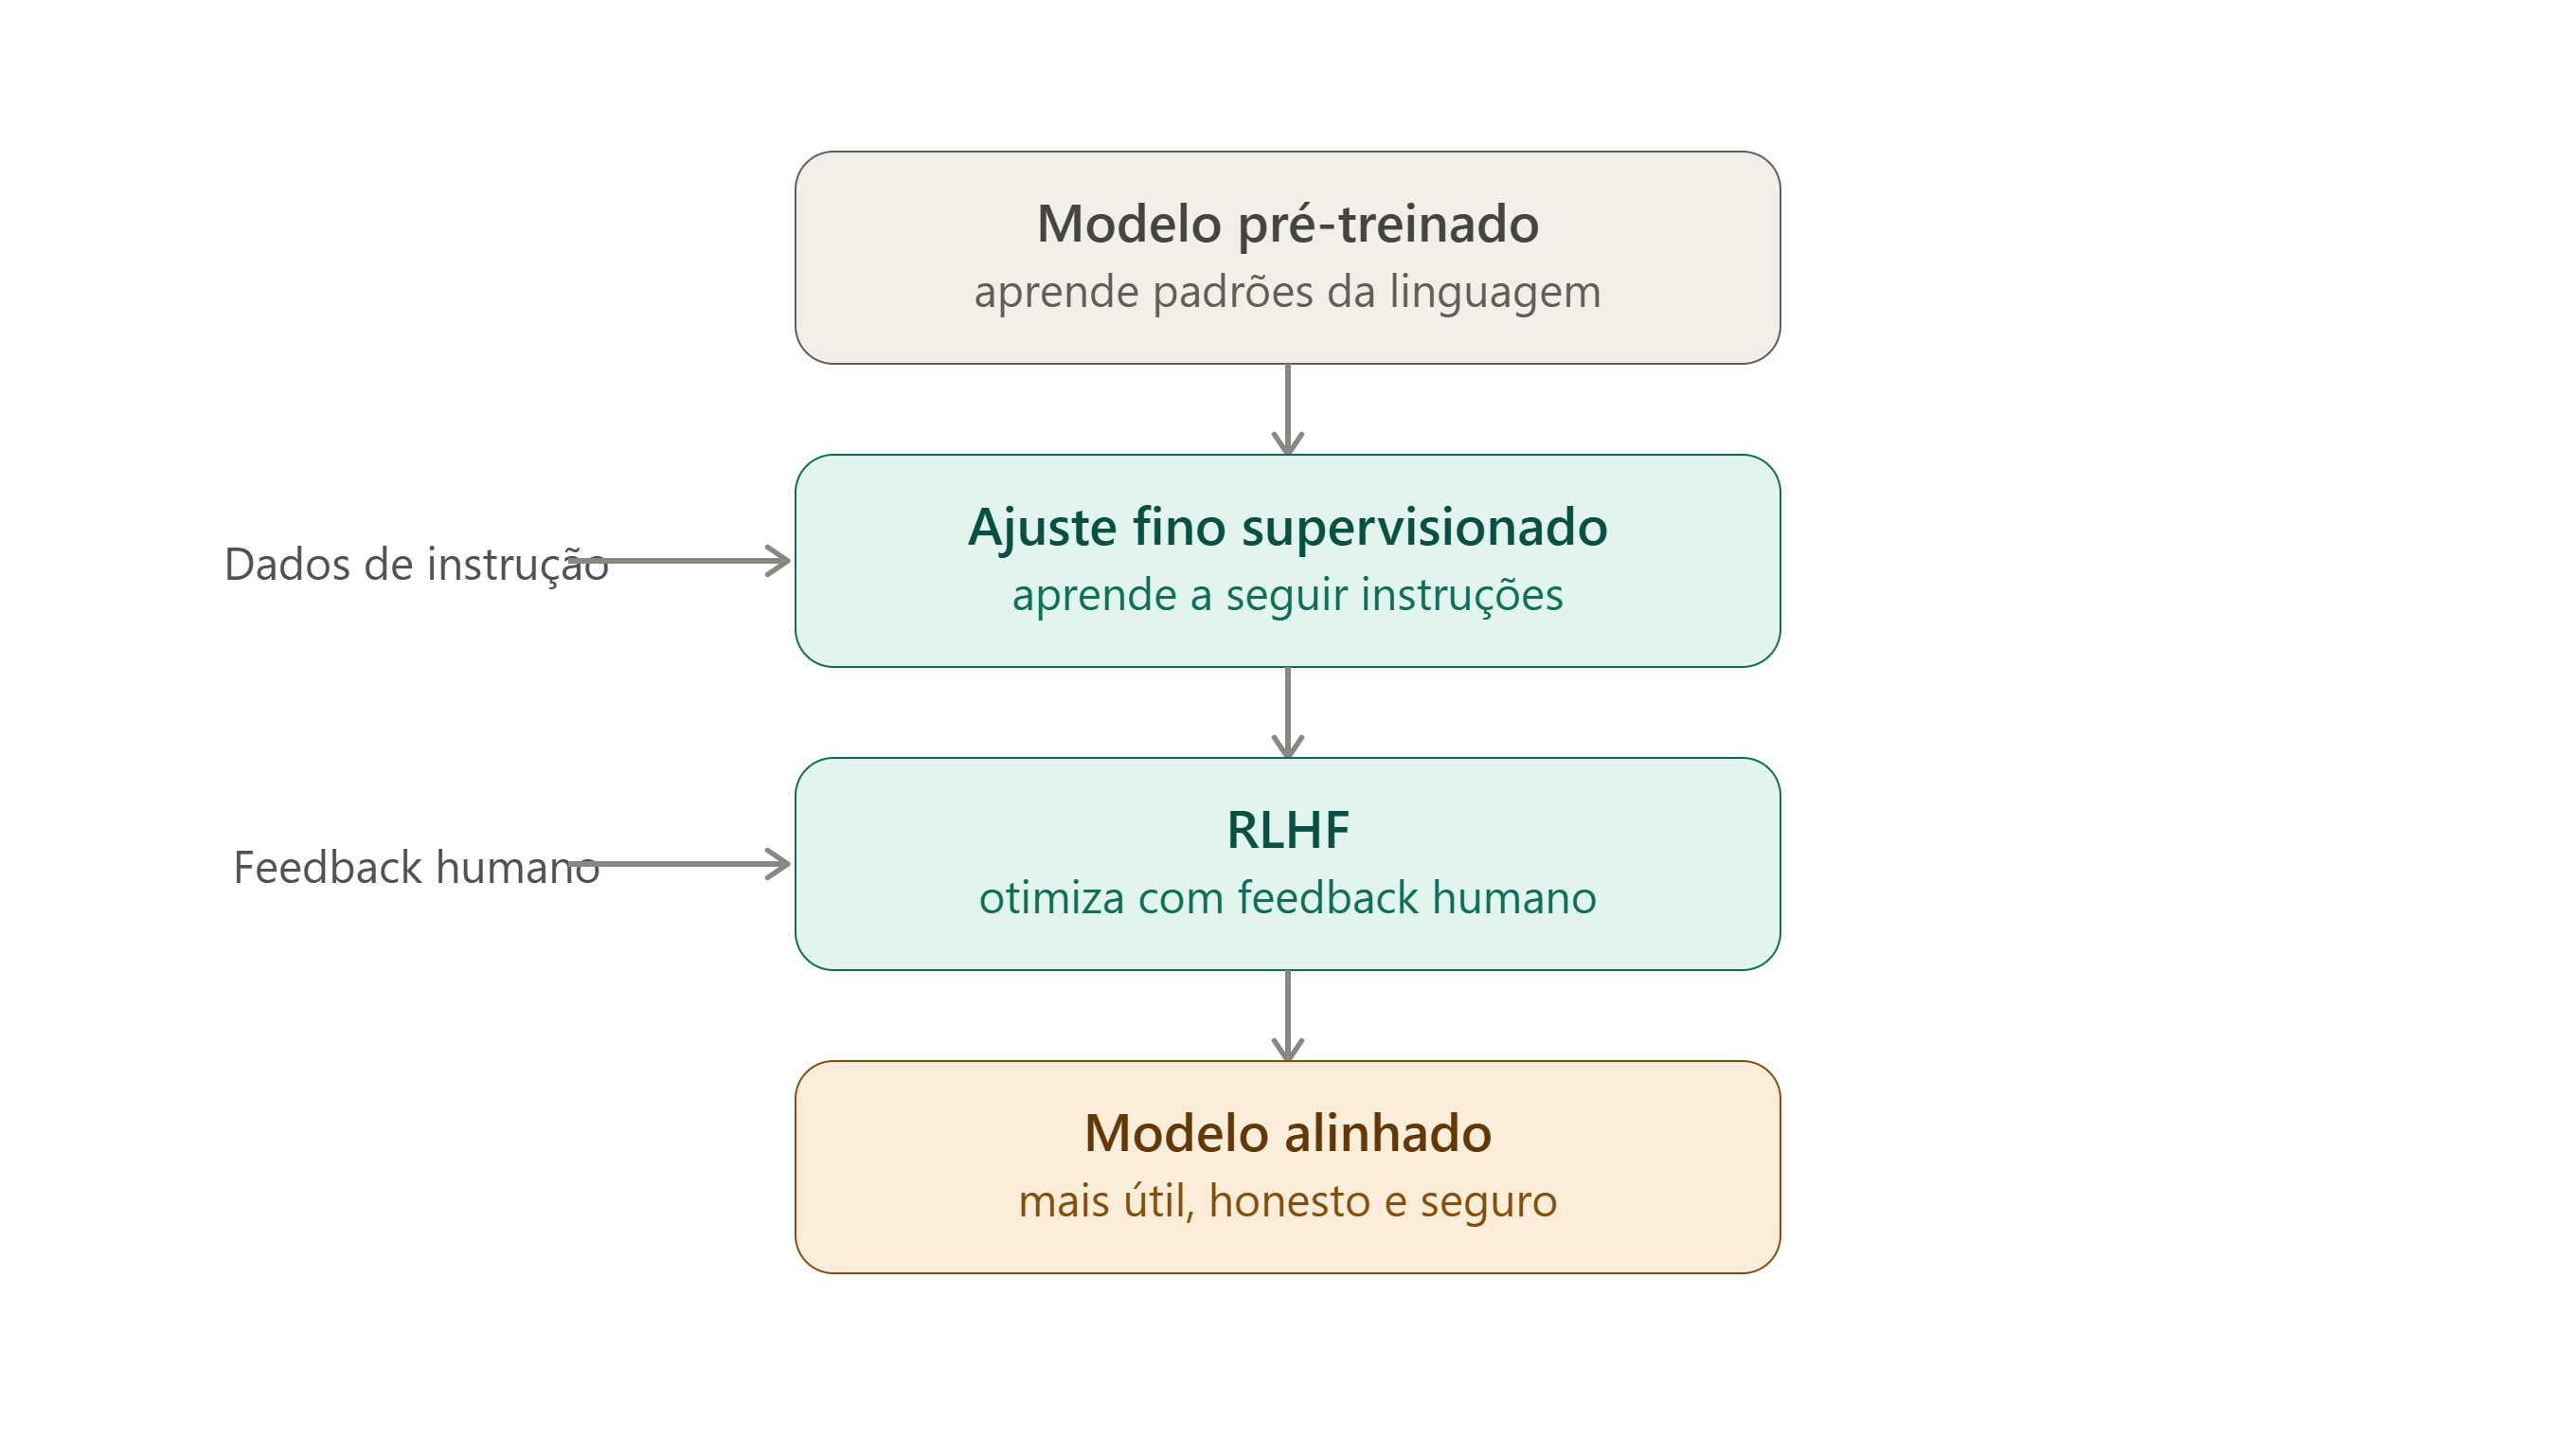
\includegraphics[scale=0.1]{fine_tuning_process.png}
    \end{column}
  \end{columns}
\end{frame}



\begin{frame}{Como você interage com o modelo}
  \begin{itemize}
    \item Você escreve um \textbf{prompt}: o modelo lê e continua a partir dos padrões que aprendeu
    \item Não é uma busca em banco de dados: é geração estatística de texto novo
    \item A \textbf{janela de contexto} é a memória de trabalho do modelo: o quanto ele consegue considerar de uma vez
  \end{itemize}
  \vspace{0.3cm}
  \begin{alertbox}{Limite prático}
    \small Sem ferramentas como busca na web, o modelo não acessa nada além do que está na conversa, incluindo eventos depois do treinamento.
  \end{alertbox}
\end{frame}

\begin{frame}{O que torna isso poderoso}
  \begin{itemize}
    \item Processa volumes enormes de informação durante o treino
    \item Aprende em contexto: se adapta a tarefas novas a partir de instruções ou exemplos no próprio prompt, sem precisar de novo treinamento
    \item Desenvolve capacidades emergentes: habilidades que aparecem com a escala, sem terem sido projetadas
  \end{itemize}
\end{frame}

% ---------------------------------------------------------------
% Capacidades e limitações: conhecer os dois lados antes de
% decidir onde a IA generativa ajuda de verdade.
% ---------------------------------------------------------------
\begin{frame}{Pontos fortes}
  \begin{itemize}
    \item Versatilidade: escreve com um tom específico, resume relatórios longos, traduz, explica temas complexos de áreas diferentes
    \item Troca de tarefa sem retreinamento: o mesmo sistema ajuda a redigir um texto e, na sequência, analisar uma planilha
    \item Mantém o fio da conversa: lembra o que foi dito antes e constrói em cima disso
    \item Conecta-se a ferramentas externas (busca na web, arquivos, outras aplicações), o que amplia bastante o que consegue ajudar
  \end{itemize}
\end{frame}

\begin{frame}{Limite: o que ela não sabe}
  \begin{notebox}{Data de corte}
    \small O modelo só conhece o mundo até a data em que foi treinado. É como alguém que entrou em um retiro sem internet: não sabe o que aconteceu depois que saiu de lá.
  \end{notebox}
  \vspace{0.3cm}
  \begin{alertbox}{Mesmo com ferramentas}
    \small Ter acesso a ferramentas externas não garante acesso à fonte certa. É como ter um colega brilhante sem acesso ao banco de dados interno da instituição: por mais competente que seja, a ajuda tem um teto.
  \end{alertbox}
\end{frame}

\begin{frame}{Limite: alucinação}
  \begin{notebox}{Definição}
    \small A IA pode afirmar algo plausível, mas incorreto, com total confiança. Diferente de um motor de busca, ela não recupera documentos: gera texto novo com base em padrões estatísticos, e às vezes erra ao juntar informações.
  \end{notebox}
  \vspace{0.3cm}
  \begin{alertbox}{A analogia}
    \small Como um amigo que conta uma história com confiança absoluta, só que os detalhes estão todos errados.
  \end{alertbox}
\end{frame}

\begin{frame}{Outras variáveis a considerar}
  \begin{itemize}
    \item \textbf{Não é determinística}: a mesma pergunta pode gerar respostas ligeiramente diferentes a cada vez
    \item \textbf{Janela de contexto}: o limite do que o modelo processa de uma vez também é uma limitação prática em documentos longos ou conversas extensas
    \item \textbf{Raciocínio em várias etapas} (matemática, lógica) é historicamente um ponto fraco, embora modelos recentes venham evoluindo nisso
  \end{itemize}
\end{frame}

% \begin{frame}{Forças complementares}
%   \begin{columns}[T,onlytextwidth]
%     \begin{column}{0.485\textwidth}
%       \begin{notebox}{O humano traz}
%         \small
%         \begin{itemize}
%           \item Pensamento crítico
%           \item Julgamento
%           \item Criatividade
%           \item Supervisão ética
%         \end{itemize}
%       \end{notebox}
%     \end{column}
%     \begin{column}{0.485\textwidth}
%       \begin{alertbox}{A IA traz}
%         \small
%         \begin{itemize}
%           \item Velocidade
%           \item Escala
%           \item Reconhecimento de padrões
%           \item Processamento de grandes volumes
%         \end{itemize}
%       \end{alertbox}
%     \end{column}
%   \end{columns}
%   \vspace{0.3cm}
%   {\small\color{graytxt} O campo muda rápido, e parte dessas limitações vem sendo mitigada. Mas algumas devem continuar por um bom tempo, daí a importância de seguir testando.}
% \end{frame}


\begin{frame}{Perguntas}
  \begin{itemize}
    \item Agora que você sabemais sobre os fundamentos técnicos da IA, isso muda como você pensa sobre a sua utilização?
    \pause
    \begin{itemize}
    \item Fluência de texto deixa de ser sinal de precisão, porque para o modelo escrever bem e estar certo são a mesma coisa (padrão estatístico), não duas competências distintas
    \item Saber da data de corte e da janela de contexto tira a expectativa de que o modelo ``já sabe'' o contexto institucional, isso vira parte do que você precisa fornecer
    \item Como o modelo se adapta só ao que está na conversa (aprendizado em contexto), refinar o prompt é reformular o que ele tem disponível, não ensinar algo permanente
    \item O cuidado com dados sensíveis é sobre o que se compartilha a cada interação, não sobre o que o modelo vai ``lembrar'' depois
  \end{itemize}
  \end{itemize}
\end{frame}


% ============================================================
% Delegação (aprofundamento) + Exercício prático
% Apenas os frames, sem preâmbulo: usa os macros já definidos no
% arquivo mestre (notebox, alertbox, dividerframe). Colar dentro
% da seção "O framework das quatro competências", no lugar do
% frame único "Delegação" já existente, antes do frame "Descrição".
% ============================================================

\dividerframe{Revisitando as competências}{}

\dividerframe{Delegação}{}

\begin{frame}{Delegação: o centro não é a IA}
  \begin{notebox}{}
    \small A base de uma boa delegação não está na IA. Está na sua própria expertise e na sua compreensão clara do que você quer alcançar.
  \end{notebox}
  \vspace{0.25cm}
  \textbf{Pergunta-guia:} o que eu exatamente quero alcançar aqui, e como é o sucesso, na prática?

  \begin{alertbox}{}
    \small Sem um objetivo claro, nem a IA mais avançada leva você a lugar nenhum.
  \end{alertbox}

  \begin{itemize}
    \item Mapear a meta e o critério de sucesso vem antes de qualquer prompt
  \end{itemize}
\end{frame}

\begin{frame}{Consciência do problema}
  \begin{notebox}{Definição}
    \small Capacidade de definir claramente seus objetivos e entender o trabalho necessário antes de trazer a IA para o processo.
  \end{notebox}
  \vspace{0.25cm}
  \textbf{Pergunta-guia:} que tipo de trabalho está em jogo aqui? Simples mas demorado, incerto, com falta de dado, ou de julgamento crítico?

  \begin{alertbox}{Ordem importa}
    \small Quem colabora bem com IA é, primeiro, especialista no próprio problema, e só depois um bom delegador de tarefas.
  \end{alertbox}
\end{frame}

\begin{frame}{Consciência de plataforma}
  \begin{notebox}{Definição}
    \small Conhecimento prático dos sistemas de IA disponíveis, e das capacidades e limites específicos de cada um.
  \end{notebox}
  \vspace{0.25cm}
  \textbf{Pergunta-guia:} você sabe quais sistemas priorizam velocidade em vez de profundidade, ou precisão em vez de criatividade?

  \begin{alertbox}{Como se desenvolve}
    \small Na prática, testando. O campo muda quase todo dia, e não existe uma ferramenta perfeita única para tudo.
  \end{alertbox}
\end{frame}

\begin{frame}{Divisão estratégica do trabalho}
  \begin{notebox}{Definição}
    \small Processo estratégico de distribuir o trabalho entre humano e IA, apoiado nos três modos já vistos: automação, aumento e agência.
  \end{notebox}
  \vspace{0.25cm}
  \begin{itemize}
    \item Que partes do fluxo se beneficiam de automação?
    \item Onde o aumento cria mais valor do que fazer sozinho ou automatizar tudo?
    \item Que áreas de julgamento crítico continuam exclusivamente humanas?
  \end{itemize}

  \begin{alertbox}{}
    \small A resposta muda de projeto para projeto, e até de etapa para etapa dentro do mesmo projeto.
  \end{alertbox}
\end{frame}

\begin{frame}{Delegação, em três elementos}
  \begin{itemize}
    \item \textbf{Consciência do problema}: entender seus objetivos e o trabalho necessário
    \item \textbf{Consciência de plataforma}: entender capacidades e limites da IA disponível
    \item \textbf{Divisão do trabalho}: distribuir estrategicamente entre você e a IA
  \end{itemize}
  \vspace{0.3cm}
  \begin{alertbox}{Ponto central}
    \small Delegar é fazer escolhas que aproveitam os pontos fortes de cada lado.
  \end{alertbox}
\end{frame}

% =========================================================
% Exercício prático
% =========================================================
\dividerframe{Exercício prático}{Analise uma tarefa com um assistente de IA}

\begin{frame}{Como fazer}
  \begin{notebox}{Passo a passo}
    \small
    \begin{enumerate}
      \item Escolha uma tarefa simples, do seu trabalho ou da sua vida pessoal (algo pequeno: redigir um e-mail, esboçar uma apresentação, planejar uma reunião ou evento)
      \item Abra uma conversa com um assistente de IA e apresente essa tarefa, pedindo ajuda para pensar em um plano de delegação
    \end{enumerate}
  \end{notebox}
  \vspace{0.3cm}
  \begin{alertbox}{Um jeito de abrir a conversa}
    \small ``Estou preparando [a tarefa] e quero pensar com você em um plano de delegação: o que eu deveria delegar a uma IA como você, e o que deveria continuar fazendo eu mesmo.''
  \end{alertbox}
\end{frame}

\begin{frame}{Perguntas para explorar juntos}
  \begin{itemize}
    \item Qual é a visão geral para essa tarefa? Como é um bom resultado?
    \item Quais são as partes de trabalho necessárias para chegar lá?
    \item Quais dessas partes exigem expertise humana, criatividade ou julgamento?
  \end{itemize}
  \vspace{0.3cm}
  \begin{notebox}{Atenção}
    \small Tenha uma conversa de verdade, não apenas troquem afirmações prontas. Vão e voltem: cada lado costuma enxergar algo que o outro não vê.
  \end{notebox}
  \vspace{0.2cm}
  \begin{alertbox}{No final}
    \small Construam juntos um plano simples de delegação, que use os pontos fortes de vocês dois.
  \end{alertbox}
\end{frame}


\dividerframe{Exercício prático}{Planejamento e delegação de projeto}

\begin{frame}{Passo 1: escolha o projeto}
  \begin{notebox}{O que escolher}
    \small Um projeto de porte médio, com várias etapas, que você possa desenvolver ao longo do restante do curso.
  \end{notebox}
  \vspace{0.3cm}
  \begin{itemize}
    \item \textbf{Substancial}: envolve tipos diferentes de tarefa
    \item \textbf{Viável}: dá para concluir em cerca de 1 hora de trabalho
    \item \textbf{Genuíno}: algo que você realmente queira criar ou realizar
  \end{itemize}
\end{frame}

\begin{frame}{Ideias de projeto (comunicação)}
  \begin{itemize}
    \item Uma apresentação envolvente sobre um tema que você domina
    \item Um post, ou série de posts, explicando um tema complexo para um público geral
    \item Uma proposta ou pitch para uma ideia que você queira levar adiante
    \item Uma bio pessoal ou profissional, com materiais de apoio
  \end{itemize}
\end{frame}

\begin{frame}{Passo 2: visão e objetivos do projeto}
  \begin{notebox}{Como fazer}
    \small Compartilhe a ideia com o Claude e deixe que ele pergunte, até vocês terem uma visão sólida do resultado final.
  \end{notebox}
  \vspace{0.3cm}
  \begin{itemize}
    \item Como é o sucesso para este projeto?
    \item O que tornaria este projeto especialmente valioso ou significativo para você?
  \end{itemize}
\end{frame}

\begin{frame}{Passo 3: análise de delegação}
  \begin{notebox}{Como no exercício anterior}
    \small Explorem o projeto pela lente da Delegação, em uma conversa de verdade, não uma lista de afirmações prontas.
  \end{notebox}
  \vspace{0.3cm}
  \begin{enumerate}
    \item Identifiquem juntos as tarefas principais do projeto
    \item Para cada tarefa, discutam uma de cada vez (próximo slide)
    \item Montem um plano de projeto com as tarefas e as decisões de delegação
    \item Salvem o plano: vocês vão voltar a ele mais adiante no curso
  \end{enumerate}
\end{frame}

\begin{frame}{Para cada tarefa, perguntem}
  \begin{itemize}
    \item Que habilidades, conhecimento ou capacidades de IA são necessárias?
    \item Que partes se beneficiam de pontos fortes exclusivamente humanos?
    \item Que partes podem aproveitar bem as capacidades da IA?
    \item Onde a colaboração teria mais impacto?
  \end{itemize}
  \vspace{0.3cm}
  \begin{alertbox}{Atenção}
    \small Desafiem suposições, peçam esclarecimentos, fiquem abertos a insights inesperados.
  \end{alertbox}
\end{frame}

\begin{frame}{Reflexão}
  \begin{itemize}
    \item Que insights surgiram da conversa de planejamento com o Claude?
    \item Qual aspecto do plano de delegação parece mais desafiador?
    \item Que informação ou habilidade adicional ajudaria a delegar melhor para a IA?
  \end{itemize}
\end{frame}

%%%%%%%%%%%%%%%%%%%%%%%%%%%%%%%%%%%%%%%%%%%%%%%%%%%%%%%%%%%%%%
\dividerframe{Descrição}{}

\begin{frame}{Descrição: além do prompt}
  \begin{notebox}{O que é}
    \small Comunicar com a IA para explicar tarefas, pedir esclarecimentos, dar contexto e guiar a interação, não só escrever prompts espertos.
  \end{notebox}
  \vspace{0.25cm}
  \textbf{Pergunta-guia:} a IA sabe o que eu quero, ou estou deixando ela adivinhar?

  \begin{alertbox}{A diferença}
    \small Pedir ``faça o jantar'' versus dar uma receita detalhada, com ingredientes e modo de preparo. A IA não lê mente.
  \end{alertbox}

  \begin{itemize}
    \item É a ponte entre a sua intenção e a capacidade da IA
  \end{itemize}
\end{frame}

\begin{frame}{Descrição de produto}
  \begin{notebox}{Definição}
    \small Capacidade de definir claramente o que você quer que a IA crie ou entregue.
  \end{notebox}
  \vspace{0.25cm}
  \textbf{Pergunta-guia:} qual é o contexto, qual o formato esperado, quem é o público e qual estilo é adequado?

  \begin{alertbox}{Não deixe a IA adivinhar}
    \small Defina requisitos explícitos, em vez de assumir que a IA já sabe o que você busca.
  \end{alertbox}
\end{frame}

\begin{frame}{Descrição de processo}
  \begin{notebox}{Definição}
    \small Capacidade de guiar como a IA aborda o seu pedido, não só o resultado final.
  \end{notebox}
  \vspace{0.25cm}
  \textbf{Pergunta-guia:} há dados específicos a usar, uma ordem a seguir, um estilo de análise ou técnica que você quer aplicada?

  \begin{alertbox}{Três formas de guiar}
    \small Uma orientação geral, como um manual; um passo a passo, como uma receita; ou uma demonstração por exemplos.
  \end{alertbox}
\end{frame}

\begin{frame}{Descrição de desempenho}
  \begin{notebox}{Definição}
    \small Capacidade de definir os aspectos comportamentais da interação com a IA.
  \end{notebox}
  \vspace{0.25cm}
  \textbf{Pergunta-guia:} você está convergindo para uma resposta específica, ou explorando possibilidades? Quer que a IA questione suas suposições, ou siga sua direção?

  \begin{alertbox}{Ponto central}
    \small Ferramentas de IA não são bancos de dados nem máquinas de vender refrigerante. São sistemas interativos, que se comportam diferente conforme o contexto, quase como pessoas.
  \end{alertbox}
\end{frame}

\begin{frame}{Descrição, em três elementos}
  \begin{itemize}
    \item \textbf{Descrição de produto}: o que você quer que a IA crie
    \item \textbf{Descrição de processo}: como a IA deve abordar o pedido
    \item \textbf{Descrição de desempenho}: como a IA deve se comportar na interação
  \end{itemize}
  \vspace{0.3cm}
  \begin{alertbox}{Ponto central}
    \small Desenvolver a descrição transforma a IA de assistência genérica em um parceiro de raciocínio afinado às suas necessidades.
  \end{alertbox}
\end{frame}


\begin{frame}{Exercício: antes e depois de um prompt ruim}
  \begin{notebox}{Como fazer}
    \small Peça ao Claude para te desafiar com prompts mal escritos, e pratique a sua Descrição para melhorá-los.
  \end{notebox}
  \vspace{0.3cm}
  \begin{enumerate}
    \item O Claude propõe prompts mal escritos para você melhorar
    \item Melhore cada um: descrição de produto (o quê), de processo (como abordar) e de desempenho (como se comportar)
    \item Converse sobre o antes e depois, e peça feedback ao Claude
    \item Depois de uns 5 minutos, troquem de papel. Observe o que o Claude acrescenta e como organiza
  \end{enumerate}
\end{frame}

\dividerframe{Prompting eficaz}{Colocando a Descrição em prática}

\begin{frame}{Seis princípios, uma prática}
  \begin{notebox}{Prompting, na prática}
    \small É como a competência de Descrição aparece no dia a dia: comunicar com clareza o que você quer, como quer que seja feito, e como quer interagir.
  \end{notebox}
  \vspace{0.3cm}
  \begin{itemize}
    \item Dar contexto
    \item Mostrar exemplos
    \item Especificar restrições de saída
    \item Dividir a tarefa em etapas
    \item Pedir para pensar antes de responder
    \item Definir papel, estilo ou tom
  \end{itemize}
\end{frame}

\begin{frame}{Dê contexto}
  \begin{notebox}{A ideia}
    \small Seja específico sobre o que você quer, por que quer, e até quem você é. Contexto reduz a adivinhação.
  \end{notebox}
  \vspace{0.3cm}
  \begin{alertbox}{Antes / depois}
    \small ``Fale sobre mudança climática'' vira ``Explique três impactos da mudança climática na agricultura em regiões tropicais, com exemplos da última década.''
  \end{alertbox}
\end{frame}

\begin{frame}{Mostre exemplos}
  \begin{notebox}{Few-shot}
    \small Mostrar exemplos do resultado que você quer é, às vezes, mais eficaz do que só descrevê-lo.
  \end{notebox}
  \vspace{0.3cm}
  \begin{alertbox}{Antes / depois}
    \small Pedir direto ``converta isto para linguagem simples'' vira mostrar dois exemplos de boas conversões antes de pedir a real.
  \end{alertbox}
\end{frame}

\begin{frame}{Especifique restrições de saída}
  \begin{notebox}{O que restringir}
    \small Formato, tamanho, linguagem de código, paleta de cores: o que for relevante para o resultado que você espera.
  \end{notebox}
  \vspace{0.3cm}
  \begin{alertbox}{Antes / depois}
    \small ``Crie um site de portfólio de arte'' vira ``crie um site de página única, com seções definidas, menu fixo e responsivo, paleta pôr do sol.''
  \end{alertbox}
\end{frame}

\begin{frame}{Divida em etapas}
  \begin{notebox}{Chain of thought}
    \small Listar os passos da tarefa ajuda o Claude a seguir o raciocínio que você quer, em vez de adivinhar o caminho.
  \end{notebox}
  \vspace{0.3cm}
  \begin{alertbox}{Antes / depois}
    \small ``Analise estes dados trimestrais'' vira ``identifique os produtos mais vendidos, compare com o trimestre anterior, destaque tendências, e sugira causas.''
  \end{alertbox}
\end{frame}

\begin{frame}{Peça para pensar antes}
  \begin{notebox}{Por quê}
    \small Dar espaço para o Claude pensar antes de responder aumenta a qualidade do resultado. Pensar antes, não explicar depois.
  \end{notebox}
  \vspace{0.3cm}
  \begin{alertbox}{Antes / depois}
    \small Perguntar direto vira acrescentar ``antes de responder, pense com cuidado nos fatores, restrições e abordagens possíveis.''
  \end{alertbox}
\end{frame}

\begin{frame}{Defina papel, estilo ou tom}
  \begin{notebox}{A pergunta}
    \small Quem você quer que a IA seja, nesta interação? Um nível de expertise, uma perspectiva, um estilo de comunicação.
  \end{notebox}
  \vspace{0.3cm}
  \begin{alertbox}{Antes / depois}
    \small ``Explique como se formam os arco-íris'' vira ``explique como se formam os arco-íris, como um professor de ciências experiente falando com uma criança de 10 anos curiosa.''
  \end{alertbox}
\end{frame}

\begin{frame}{A técnica mais poderosa}
  \begin{notebox}{Peça ajuda para melhorar o prompt}
    \small Quando não souber como pedir algo, descreva a situação ao Claude e peça que ele escreva ou melhore o prompt para você.
  \end{notebox}
  \vspace{0.3cm}
  \begin{alertbox}{Peça assim}
    \small ``Estou tentando te pedir ajuda com [objetivo], mas não sei bem como formular. Pode me ajudar a montar um prompt melhor pra isso?''
  \end{alertbox}
\end{frame}

\begin{frame}{O que funciona, e o que evitar}
  \begin{columns}[T,onlytextwidth]
    \begin{column}{0.485\textwidth}
      \begin{notebox}{Padrões que funcionam}
        \small
        \begin{itemize}
          \item Começar com uma visão clara da tarefa
          \item Incluir formato e exemplos
          \item Dar contexto rico e relevante
        \end{itemize}
      \end{notebox}
    \end{column}
    \begin{column}{0.485\textwidth}
      \begin{alertbox}{Erros comuns}
        \small
        \begin{itemize}
          \item Assumir que o Claude lê mentes
          \item Misturar tarefas não relacionadas
          \item Não dar feedback sobre respostas anteriores
        \end{itemize}
      \end{alertbox}
    \end{column}
  \end{columns}
\end{frame}

\begin{frame}{Reflexão}
  \begin{itemize}
    \item Qual das seis técnicas você acha que mais melhoraria suas interações atuais com a IA?
    \item Pense em uma interação recente que não atendeu ao que você precisava. Que técnicas poderiam ter mudado o resultado?
    \item Como essas técnicas se conectam com a competência de Descrição do framework de Fluência em IA?
  \end{itemize}
  \vspace{0.3cm}
  \begin{alertbox}{Para treinar}
    \small Se quiser, revisite o exercício ``Antes e depois de um prompt ruim'' e aplique esses princípios.
  \end{alertbox}
\end{frame}

\dividerframe{Discernimento}{}

\begin{frame}{Discernimento: o contraponto da Descrição}
  \begin{notebox}{O que é}
    \small Capacidade de avaliar criticamente o que a IA produz, como ela chega lá, e como se comporta. É o outro lado da Descrição.
  \end{notebox}
  \vspace{0.25cm}
  \textbf{Pergunta-guia:} o que voltou realmente atende ao que eu precisava?

  \begin{alertbox}{Exige duas coisas}
    \small Expertise no assunto, para julgar qualidade, e entendimento de como sistemas de IA costumam falhar.
  \end{alertbox}
\end{frame}

\begin{frame}{Discernimento de produto}
  \begin{notebox}{Definição}
    \small Capacidade de julgar a precisão e o valor do que a IA produziu.
  \end{notebox}
  \vspace{0.25cm}
  \begin{alertbox}{Perguntas para fazer}
    \small Isso está correto? É adequado para o meu público e o meu propósito? Resolve o problema que eu tinha?
  \end{alertbox}
\end{frame}

\begin{frame}{Discernimento de processo}
  \begin{notebox}{Definição}
    \small Avaliar não só o que a IA produziu, mas como ela chegou lá: erros de lógica, lapsos de atenção, raciocínio circular.
  \end{notebox}
  \vspace{0.25cm}
  \begin{alertbox}{Exemplo}
    \small Você pede para expandir uma de cinco estruturas propostas para um texto. Depois de várias rodadas, elementos das ideias já rejeitadas voltam a aparecer.
  \end{alertbox}
\end{frame}

\begin{frame}{Discernimento de desempenho}
  \begin{notebox}{Definição}
    \small Avaliar e guiar como a IA se comporta durante a interação, não só o trabalho em si.
  \end{notebox}
  \vspace{0.25cm}
  \begin{alertbox}{Exemplo}
    \small A IA faz perguntas demais quando você queria respostas diretas, ou é breve demais quando você precisava de profundidade.
  \end{alertbox}
\end{frame}

\begin{frame}{Dar feedback que funciona}
  \begin{notebox}{O que inclui}
    \small Dizer qual é o problema, explicar por que é um problema, dar sugestões concretas, revisar instruções ou exemplos.
  \end{notebox}
  \vspace{0.25cm}
  \begin{alertbox}{Nem sempre é descrição}
    \small Às vezes o problema não é como você descreveu, é a ferramenta ou a abordagem errada. Aí a questão é repensar a delegação.
  \end{alertbox}
\end{frame}

\begin{frame}{Discernimento, em três elementos}
  \begin{itemize}
    \item \textbf{Discernimento de produto}: a precisão e o valor do resultado
    \item \textbf{Discernimento de processo}: a qualidade do caminho até o resultado
    \item \textbf{Discernimento de desempenho}: a qualidade da interação em si
  \end{itemize}
  \vspace{0.3cm}
  \begin{alertbox}{Ponto central}
    \small Descrição e discernimento formam um ciclo contínuo: um comunica o que você quer, o outro avalia se funcionou.
  \end{alertbox}
\end{frame}

\begin{frame}{Reflexão}
  \begin{itemize}
    \item Dos três tipos, produto, processo ou desempenho, qual você mais costuma deixar passar batido?
    \item Que expertise sua, no seu campo, mais ajuda você a perceber quando a IA está errada com segurança?
  \end{itemize}
\end{frame}

\dividerframe{Diligência}{}

% \begin{frame}{Diligência: responsabilidade em cada interação}
%   \begin{notebox}{O que é}
%     \small Assumir a responsabilidade pelas suas interações com IA: rigor, transparência e prestação de contas, não só produtividade.
%   \end{notebox}
%   \vspace{0.3cm}
%   \begin{alertbox}{Como dirigir um carro}
%     \small Não basta chegar do ponto A ao B com eficiência. Também importam a segurança, as regras, e o efeito sobre os outros na estrada.
%   \end{alertbox}
% \end{frame}

% \begin{frame}{As perguntas que abrem a diligência}
%   \begin{itemize}
%     \item Quais são as implicações de trabalhar com essa IA?
%     \item Quem pode ser afetado pelo que é criado, pela colaboração em si, ou por um erro que passou despercebido?
%     \item Quem tem acesso aos dados usados para produzir esse resultado?
%     \item Essa interação está alinhada com padrões éticos e com os meus valores?
%   \end{itemize}
% \end{frame}

% \begin{frame}{Diligência de criação}
%   \begin{notebox}{Definição}
%     \small Ser crítico e intencional sobre quais sistemas de IA você usa, e como você os usa.
%   \end{notebox}
%   \vspace{0.25cm}
%   \begin{itemize}
%     \item Como esse sistema foi treinado, e com que dados?
%     \item Quem é dono dos dados que estou inserindo, e quem pode ter acesso a eles?
%     \item Como estou protegendo a privacidade e a segurança, minha e de outros?
%     \item Isso está alinhado aos meus valores, ou às políticas da minha organização?
%   \end{itemize}
% \end{frame}

% \begin{frame}{Diligência de transparência}
%   \begin{notebox}{Definição}
%     \small Ser aberto e preciso sobre a participação da IA, com todos que precisam saber disso.
%   \end{notebox}
%   \vspace{0.25cm}
%   \begin{itemize}
%     \item Quem precisa saber do papel da IA aqui?
%     \item Como e quando devo comunicar isso?
%     \item Que nível de detalhe faz sentido compartilhar?
%   \end{itemize}
%   \vspace{0.2cm}
%   \begin{alertbox}{Exemplo}
%     \small Usou a IA numa proposta em equipe? Avisar quais partes tiveram ajuda da IA mantém a colaboração honesta.
%   \end{alertbox}
% \end{frame}

% \begin{frame}{Diligência de publicação}
%   \begin{notebox}{Definição}
%     \small Responsabilidade pelo que você usa ou compartilha, depois que a IA ajudou a criar.
%   \end{notebox}
%   \vspace{0.25cm}
%   \begin{itemize}
%     \item Verificar cada fato e cada fonte
%     \item Checar vieses
%     \item Garantir direitos de uso
%   \end{itemize}
%   \vspace{0.2cm}
%   \begin{alertbox}{Exemplo}
%     \small Um jornalista que usa IA para rascunhar uma matéria ainda cumpre os mesmos padrões de sempre, antes de publicar.
%   \end{alertbox}
% \end{frame}

% \begin{frame}{Diretrizes pessoais}
%   \begin{notebox}{Por que importa}
%     \small Contextos e públicos diferentes têm expectativas diferentes. Vale desenvolver diretrizes próprias, alinhadas aos seus valores.
%   \end{notebox}
%   \vspace{0.25cm}
%   \begin{alertbox}{Fique atento}
%     \small Em contextos profissionais, conheça as políticas da sua organização. As regras sobre IA ainda estão em formação.
%   \end{alertbox}
% \end{frame}

% \begin{frame}{Diligência, em três elementos}
%   \begin{itemize}
%     \item \textbf{Diligência de criação}: escolher e usar sistemas de IA com critério
%     \item \textbf{Diligência de transparência}: ser aberto sobre o papel da IA
%     \item \textbf{Diligência de publicação}: responder pela precisão do que você compartilha
%   \end{itemize}
%   \vspace{0.3cm}
%   \begin{alertbox}{Ponto central}
%     \small Você, não a IA, é quem responde pelo que cria, usa e compartilha.
%   \end{alertbox}
% \end{frame}

\begin{frame}{Diligência: responsabilidade em cada interação}
  \begin{notebox}{O que é}
    \small Assumir a responsabilidade pelas suas interações com IA: rigor, transparência e prestação de contas, não só produtividade.
  \end{notebox}
  \vspace{0.3cm}
  \begin{alertbox}{Como dirigir um carro}
    \small Não basta chegar do ponto A ao B com eficiência. Também importam a segurança, as regras, e o efeito sobre os outros na estrada.
  \end{alertbox}
\end{frame}

\begin{frame}{As perguntas que abrem a diligência}
  \begin{itemize}
    \item Quais são as implicações de trabalhar com essa IA?
    \item Quem pode ser afetado pelo que é criado, pela colaboração em si, ou por um erro que passou despercebido?
    \item Quem tem acesso aos dados usados para produzir esse resultado?
    \item Essa interação está alinhada com padrões éticos e com os meus valores?
  \end{itemize}
\end{frame}

\begin{frame}{Diligência de criação}
  \begin{notebox}{Definição}
    \small Ser crítico e intencional sobre quais sistemas de IA você usa, e como você os usa.
  \end{notebox}
  \vspace{0.25cm}
  \begin{itemize}
    \item Como esse sistema foi treinado, e com que dados?
    \item Quem é dono dos dados que estou inserindo, e quem pode ter acesso a eles?
    \item Como estou protegendo a privacidade e a segurança, minha e de outros?
    \item Isso está alinhado aos meus valores, ou às políticas da minha organização?
  \end{itemize}
\end{frame}

\begin{frame}{Diligência de transparência}
  \begin{notebox}{Definição}
    \small Ser aberto e preciso sobre a participação da IA, com todos que precisam saber disso.
  \end{notebox}
  \vspace{0.25cm}
  \begin{itemize}
    \item Quem precisa saber do papel da IA aqui?
    \item Como e quando devo comunicar isso?
    \item Que nível de detalhe faz sentido compartilhar?
  \end{itemize}
  \vspace{0.2cm}
  \begin{alertbox}{Exemplo}
    \small Usou a IA numa proposta em equipe? Avisar quais partes tiveram ajuda da IA mantém a colaboração honesta.
  \end{alertbox}
\end{frame}

\begin{frame}{Diligência de publicação}
  \begin{notebox}{Definição}
    \small Responsabilidade pelo que você usa ou compartilha, depois que a IA ajudou a criar.
  \end{notebox}
  \vspace{0.25cm}
  \begin{itemize}
    \item Verificar cada fato e cada fonte
    \item Checar vieses
    \item Garantir direitos de uso
  \end{itemize}
  \vspace{0.2cm}
  \begin{alertbox}{Exemplo}
    \small Um jornalista que usa IA para rascunhar uma matéria ainda cumpre os mesmos padrões de sempre, antes de publicar.
  \end{alertbox}
\end{frame}

\begin{frame}{Diretrizes pessoais}
  \begin{notebox}{Por que importa}
    \small Contextos e públicos diferentes têm expectativas diferentes. Vale desenvolver diretrizes próprias, alinhadas aos seus valores.
  \end{notebox}
  \vspace{0.25cm}
  \begin{alertbox}{Fique atento}
    \small Em contextos profissionais, conheça as políticas da sua organização. As regras sobre IA ainda estão em formação.
  \end{alertbox}
\end{frame}

\begin{frame}{Diligência, em três elementos}
  \begin{itemize}
    \item \textbf{Diligência de criação}: escolher e usar sistemas de IA com critério
    \item \textbf{Diligência de transparência}: ser aberto sobre o papel da IA
    \item \textbf{Diligência de publicação}: responder pela precisão do que você compartilha
  \end{itemize}
  \vspace{0.3cm}
  \begin{alertbox}{Ponto central}
    \small Você, não a IA, é quem responde pelo que cria, usa e compartilha.
  \end{alertbox}
\end{frame}

\begin{frame}{Reflexão}
  \begin{itemize}
    \item Qual aspecto da Diligência, criação, transparência ou publicação, você acha mais desafiador, e por quê?
    \item Como a sua abordagem de Diligência muda conforme o contexto: pessoal, acadêmico, profissional?
    \item Como reconhecer o papel da IA no seu trabalho muda a forma como os outros o percebem?
    \item Que considerações éticas surgiram no seu projeto que você não tinha previsto?
    \item Que diretrizes pessoais você poderia desenvolver para uma colaboração responsável com IA daqui pra frente?
  \end{itemize}
\end{frame}

\dividerframe{Exercício prático}{Criando uma declaração de diligência}

\begin{frame}{Passo 1: entenda a declaração}
  \begin{notebox}{O que é}
    \small Um reconhecimento transparente do papel da IA no seu trabalho, com um compromisso de responsabilidade pelo resultado final.
  \end{notebox}
  \vspace{0.3cm}
  \begin{alertbox}{Modelo}
    \small ``Na criação deste projeto, colaborei com o Claude em [tarefas específicas]. Todo o conteúdo gerado passou por revisão minha. Assumo total responsabilidade pelo conteúdo, sua precisão e apresentação.''
  \end{alertbox}
\end{frame}

\begin{frame}{Passo 2: reflita, diligência de criação}
  \begin{itemize}
    \item Quais sistemas de IA você escolheu usar, e por quê?
    \item Que dados ou informações você compartilhou com a IA?
    \item Houve considerações de privacidade, segurança ou ética nessas escolhas?
  \end{itemize}
\end{frame}

\begin{frame}{Passo 2: reflita, diligência de transparência}
  \begin{itemize}
    \item Quem é o público do resultado do seu projeto?
    \item Que expectativas ele pode ter sobre a divulgação do uso de IA?
    \item Como, especificamente, a IA contribuiu para partes diferentes do seu trabalho?
  \end{itemize}
\end{frame}

\begin{frame}{Passo 2: reflita, diligência de publicação}
  \begin{itemize}
    \item Que passos você tomou para verificar a precisão das contribuições da IA?
    \item Como você garantiu que o resultado final atende aos seus padrões?
    \item Que responsabilidade você assume pelo produto final?
  \end{itemize}
\end{frame}

\begin{frame}{Passo 3: redija sua declaração}
  \begin{notebox}{Como fazer}
    \small Abra uma conversa com o Claude, compartilhe suas reflexões do Passo 2, e redijam juntos a declaração.
  \end{notebox}
  \vspace{0.3cm}
  \begin{alertbox}{A declaração deve cobrir}
    \small Quais sistemas de IA você usou, como a IA contribuiu, o processo de revisão, sua responsabilidade pelo resultado, e considerações específicas do contexto.
  \end{alertbox}
\end{frame}

\begin{frame}{Passo 4: adicione ao projeto}
  \begin{notebox}{Onde colocar}
    \small Quando terminar o projeto, inclua a sua declaração de diligência em um lugar apropriado: rodapé, apêndice, ou metadados.
  \end{notebox}
\end{frame}

\begin{frame}{}
  % Sugestão de síntese: ajuste para a formulação que preferir.
  \begin{center}
    \vspace{0.4cm}
    {\Large\color{navy}\bfseries Fluência em IA não é usar um monte de ferramentas,\\ é saber quando delegar, como descrever\\ e quando desconfiar.}
    \vspace{0.4cm}
  \end{center}
\end{frame}

\begin{frame}[allowframebreaks]{Referências}
  \small
  \begin{itemize}
    \item Anthropic Academy. \textit{AI Fluency: Framework \& Foundations}. Curso desenvolvido com Joseph Feller (University College Cork) e Rick Dakan (Ringling College). \url{https://www.anthropic.com/ai-fluency}
  \end{itemize}
\end{frame}

\dividerframe{Obrigado!}{Perguntas?}



% =========================================================
\section{Ética como parte do fluxo}
% =========================================================
\dividerframe{Ética como parte do fluxo}{Não é uma etapa extra no fim, é parte de como se decide usar a ferramenta}

\begin{frame}{Três perguntas éticas, em cada uso}
  \begin{itemize}
    \item \textbf{Criação}: por que escolhi esta ferramenta para esta tarefa, e não outra abordagem?
    \item \textbf{Transparência}: as pessoas que vão receber este material sabem que a IA participou?
    \item \textbf{Responsabilização}: quando este material sai daqui, de quem é a assinatura?
  \end{itemize}
  \vspace{0.3cm}
  \begin{notebox}{Ponto central}
    \small Nenhuma dessas três perguntas tem uma resposta fixa: o que é aceitável varia conforme o contexto (uma nota interna não é uma matéria assinada, e um rascunho não é uma peça final).
  \end{notebox}
\end{frame}

\begin{frame}{Normas variam por contexto}
  \begin{itemize}
    \item O que vale para um rascunho interno não vale para uma publicação institucional
    \item O que vale para um post de redes sociais não vale para uma nota oficial
    \item Cada equipe de comunicação precisa decidir suas próprias linhas, com base nesses princípios
  \end{itemize}
  \vspace{0.3cm}
  % PREENCHER: se a UFOP já tiver alguma diretriz institucional de uso de IA
  % na comunicação, este é o lugar para citá-la.
  \begin{alertbox}{Para discussão}
    \small Esta universidade já tem, ou deveria ter, uma política própria de uso de IA na comunicação institucional?
  \end{alertbox}
\end{frame}

% =========================================================
\section{Ferramentas: bom uso, mau uso}
% =========================================================
\dividerframe{Ferramentas na prática da comunicação}{Bom uso e mau uso: o centro desta conversa}

\begin{frame}{Como avaliar uma ferramenta antes de adotar}
  \begin{itemize}
    \item Para que tarefa específica ela serve aqui, nesta equipe?
    \item O que ela decide sozinha, e o que continua exigindo uma pessoa?
    \item Onde os dados que ela usa ou produz ficam armazenados?
    \item Quem checa o resultado antes de ele sair da equipe?
    \item O que muda se essa ferramenta ficar indisponível amanhã?
  \end{itemize}
\end{frame}

% ---------------------------------------------------------------
% Os quatro slides abaixo usam a macro \ferramentaframe.
% Os itens estão com exemplos de ponto de partida: troque pelos
% casos e ferramentas que fizerem mais sentido para esta equipe.
% Para acrescentar uma quinta categoria, copie um destes blocos.
% ---------------------------------------------------------------

\ferramentaframe{Redação e edição de texto}
  {Assistentes de escrita de uso geral (Claude, ChatGPT, Gemini e afins)}
  {
    \item Rascunhar uma primeira versão de nota ou release
    \item Adaptar o mesmo texto para públicos diferentes
    \item Revisar clareza, tom e concisão
  }
  {
    \item Publicar sem revisão humana
    \item Usar para decidir o que a instituição vai dizer
    \item Inserir dados ou nomes sem conferir a fonte
  }

\ferramentaframe{Imagem, áudio e vídeo generativos}
  {Geração de imagem, voz sintética e edição assistida por IA}
  % PREENCHER: nomes de ferramentas específicas usadas por esta equipe
  {
    \item Ilustrações genéricas para posts e materiais internos
    \item Rascunhos visuais para testar uma ideia de campanha
  }
  {
    \item Retratar pessoas reais ou situações que pareçam reais sem identificação clara
    \item Usar como se fosse fotografia jornalística
  }

\ferramentaframe{Pesquisa, transcrição e síntese}
  {Transcrição de entrevistas, resumo de reuniões e apoio a levantamentos}
  {
    \item Transcrever entrevistas e reuniões longas
    \item Resumir documentos extensos para uma primeira leitura
  }
  {
    \item Tratar o resumo como substituto da leitura da fonte original
    \item Citar dado ou estatística sem confirmar de onde veio
  }

\ferramentaframe{Atendimento e relacionamento com o público}
  {Chatbots e respostas automatizadas em canais institucionais}
  {
    \item Responder perguntas frequentes e bem delimitadas
    \item Direcionar o público para o canal humano certo
  }
  {
    \item Deixar a IA responder sozinha em situações sensíveis ou de crise
    \item Simular uma pessoa quando quem está respondendo é um sistema
  }

\begin{frame}{Casos e experiências da equipe}
  % PREENCHER no dia: espaço para os colegas de comunicação
  % compartilharem ferramentas e casos reais (conecta com a parte
  % prática do evento).
  \begin{itemize}
    \item Qual ferramenta de IA já faz parte da rotina desta equipe?
    \item O que funcionou melhor do que o esperado?
    \item O que quase deu errado, e o que se aprendeu com isso?
  \end{itemize}
\end{frame}

% =========================================================
\section{Possibilidades}
% =========================================================
\dividerframe{Possibilidades}{Onde a IA amplia o trabalho da comunicação}

\begin{frame}{Produtividade e escala}
  \begin{itemize}
    \item Produzir mais variações de um mesmo material em menos tempo
    \item Liberar tempo da equipe para o que exige julgamento humano
    \item Adaptar um mesmo conteúdo para vários formatos e canais
  \end{itemize}
\end{frame}

\begin{frame}{Acessibilidade e inclusão}
  \begin{itemize}
    \item Gerar versões em linguagem simples de textos institucionais complexos
    \item Apoiar tradução e adaptação para diferentes públicos
    \item Transcrição e legendagem de conteúdo em áudio e vídeo
  \end{itemize}
\end{frame}

\begin{frame}{Escuta e personalização}
  \begin{itemize}
    \item Analisar grandes volumes de comentários e menções nas redes
    \item Identificar padrões e temas recorrentes na percepção pública
    \item Personalizar comunicação para diferentes públicos institucionais
  \end{itemize}
\end{frame}

\begin{frame}{Novos formatos narrativos}
  \begin{itemize}
    \item Explorar formatos que antes exigiam equipes maiores (vídeo curto, podcast, infográfico)
    \item Testar rapidamente diferentes abordagens antes de investir na produção final
  \end{itemize}
\end{frame}

% =========================================================
\section{Limites e riscos}
% =========================================================
\dividerframe{Limites e riscos}{Reais, mas não são motivo para não usar, são motivo para usar com discernimento}

\begin{frame}{Quatro riscos recorrentes}
  \begin{itemize}
    \item \textbf{Alucinação}: a IA pode inventar fatos, citações e fontes com total confiança
    \item \textbf{Viés}: o resultado reflete os padrões dos dados de treino, não neutralidade
    \item \textbf{Opacidade}: nem sempre é possível explicar por que a IA chegou a uma resposta
    \item \textbf{Dependência}: usar demais sem checar pode erodir a própria capacidade crítica da equipe com o tempo
  \end{itemize}
\end{frame}

% =========================================================
\section{Síntese}
% =========================================================
\dividerframe{Para fechar}{}

\begin{frame}{A tese, em uma frase}
  % Sugestão de síntese: ajuste para a formulação que preferir.
  \begin{center}
    \vspace{0.4cm}
    {\Large\color{navy}\bfseries Fluência em IA não é usar mais ferramentas,\\ é saber quando delegar, como descrever\\ e quando desconfiar.}
    \vspace{0.4cm}
  \end{center}
\end{frame}

\begin{frame}{Agora, a palavra é de vocês}
  \begin{itemize}
    \item Quais ferramentas de IA já fazem parte do dia a dia da comunicação nesta universidade?
    \item O que essa equipe já sabe sobre uso de IA que vale compartilhar?
    \item Onde vocês sentem falta de uma diretriz clara?
  \end{itemize}
\end{frame}

\begin{frame}[allowframebreaks]{Referências}
  \small
  \begin{itemize}
    \item Anthropic Academy. \textit{AI Fluency: Framework \& Foundations}. Curso desenvolvido com Joseph Feller (University College Cork) e Rick Dakan (Ringling College). \url{https://www.anthropic.com/ai-fluency}
  \end{itemize}
\end{frame}

\end{document}
